\chapter{Abastecimiento de agua CTE DB-HS4}
\section{Propósito de la instalación}
Hacer llegar el agua a cada punto de consumo en un edificio.

\section{Marco normativo}
\subsection{Marco normativo}
Atendiendo al ahorro y la eficiencia en el consumo, la gestión y el uso del agua está regulada por:
\begin{itemize}
    \item CTE, Código Técnico de la Edificación
    \begin{itemize}
        \item Documento Básico HS 4 Suministro de agua
    \end{itemize}
    \item Normas UNE
    \begin{itemize}
        \item UNE 149201 Dimensionado de instalaciones de agua para consumo humano dentro de los edificios.
    \end{itemize}
\end{itemize}

\subsection{Estructura del CTE}
\begin{itemize}
    \item Parte I: Exigencias básicas
    \begin{itemize}
        \item Qué requisitos básicos de seguridad y habitabilidad deben cumplir los edificios.
    \end{itemize}
    \item Parte II: Documentos Básicos (DB)
    \begin{itemize}
        \item Reglas y procedimientos para cumplir esas exigencias básicas.
        \item Hay 3 DB de Seguridad
        \begin{itemize}
            \item Seguridad estructural (DB SE)
            \item Seguridad en caso de incendio (DB SI)
            \item Seguridad de utilización y accesibilidad (DB SUA)
        \end{itemize}
        \item Y otras 3 DB de Habitabilidad
        \begin{itemize}
            \item Salubridad (DB HS)
            \item Protección frente a ruido (DB HR)
            \item Ahorro de energía (DB HE)
        \end{itemize}
    \end{itemize}
\end{itemize}

\begin{figure}[h]
    \centering
    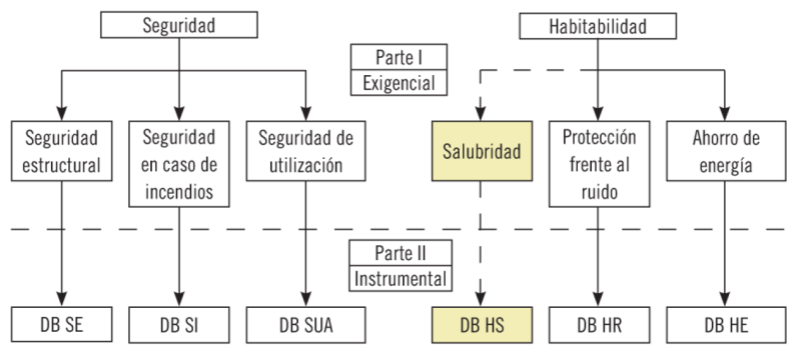
\includegraphics[width=\linewidth]{Imagenes/Estructura del CTE.png}
    \caption{Estructura del CTE.}
\end{figure}

\subsection{DB-HS (salubridad)}
Establece las reglas y los procedimientos que permiten cumplir las exigencias básicas de salubridad. Tiene 5 secciones:
\begin{enumerate}
    \item Protección frente a la humedad (DB HS 1)
    \item Recogida y evacuación de residuos (DB HS 2)
    \item Calidad del aire interior (DB HS 3)
    \item Suminsitro de agua (DB HS 4)
    \item Evacuación de aguas (DB HS 5)
\end{enumerate}

\subsubsection{DB-HS4 (Suministro de agua)}
Los edificios dispondrán de medios adecuados para suministrar al equipamiento higiénico previsto de agua apta para el consumo de forma sostenible, aportando caudales suficientes para su funcionamiento, sin alteración de las propiedades de aptitud para el consumo impidiendo los posibles retornos que puedan contaminar la red, incorporando medios que permitan el ahorro y el control del agua.

Los equipos de producción de ACS dotasdos de sistemas de acumulación y los puntos terminales de utilización tendrán unas características tales que eviten el desarrollo de gérmenes patógenos.

\begin{figure}[h]
    \centering
    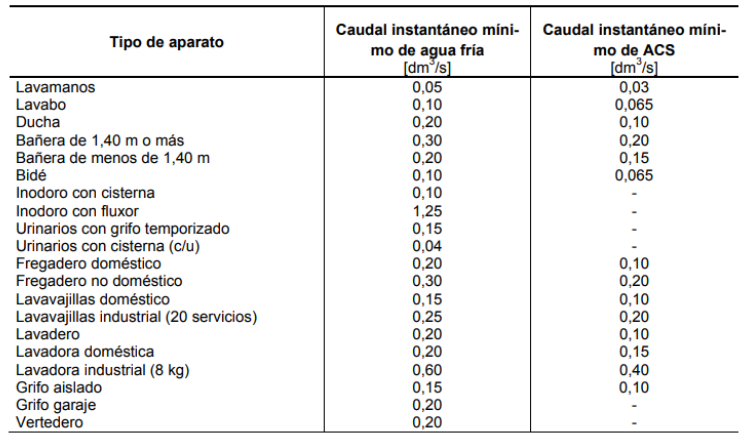
\includegraphics[width=\linewidth]{Imagenes/DBHS4 - Caudales mínimos.png}
    \caption{Caudal instantáneo mínimo para cada tipo de aparato}
\end{figure}

En los puntos de consumo la presión mínima debe ser:
\begin{itemize}
    \item $100\ kPa$ para grifos comunes
    \item $150 kPa$ para fluxores y calentadores
\end{itemize}
La presión en cualquier punto de consumo no debe superar $500\ kPa$.
La temperatura de ACS en los puntos de consumo debe estar comprendida entre $50 ^\circ C$ y $65 ^\circ C$excepto en las instalaciones ubicadas en edificios dedicados a uso exclusivo de vivienda.

\subsection{Otras normativas}
\begin{itemize}
    \item Código Técnico de la Edificación (CTE)
    \item Legislación autonómica
    \item Ordenanzas municipales
    \item Pliegos de prescripciones técnicas (suministrador)
    \begin{itemize}
        \item CYII, suministros de agua
    \end{itemize}
    \item Reglamentos de suministro de agua
\end{itemize}

\begin{figure}[h]
    \centering
    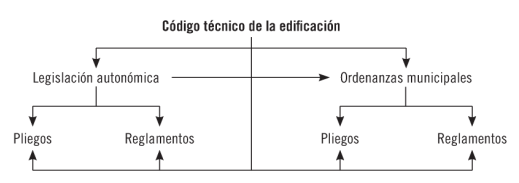
\includegraphics[width=\linewidth]{Imagenes/normativas.png}
    \caption{Normativas}
\end{figure}

\section{Diseño conceptual}
Vivienda unifamiliar:
\begin{itemize}
    \item AFCH (Agua Fría de Consumo Humano)
    \item ACS (Agua Caliente Sanitaria)
    \item Agua para calefacción (individual)
    \item Agua para riego
\end{itemize}

Vivienda plurifamiliar:
\begin{itemize}
    \item AFCH (presión adicional)
    \item ACS (complemento por energía solar térmica)
    \item Calefacción (sistema centralizado)
    \item Red de riego exterior
    \item Toma de incendios para los bomberos (hidrante)
\end{itemize}

Edificio de oficinas:
\begin{itemize}
    \item AFCH (presión adicional)
    \item ACS (complemento energía solar)
    \item Agua para calefacción (sistema central)
    \item Suministro agua para PCI activa (rociadores, etc.)
    \item Riego, limpieza, servicios auxiliares
    \item Comedores, personal
\end{itemize}

Edificio industrial:
\begin{itemize}
    \item AFCH (presión adicional y auto-abastecimiento)
    \item ACS (complemento energía solar)
    \item Calefacción (centralizada)
    \item Suministro agua para PCI activa (rociadores)
    \item Comedores, personal
    \item Agua de proceso
\end{itemize}

Edificio industrial en zona aislada:
\begin{itemize}
    \item AFCH (presión adicional y auto-abastecimiento)
    \item ACS (complemento energía solar)
    \item Calefacción (radiadores por agua)
    \item Suministro agua para PCI activa
    \item Agua de proceso
    \item Posible necesidad de captación
\end{itemize}

\section{Elementos de la instalación}
\subsection{Componentes principales}
\begin{itemize}
    \item Acometida. Conecta la red exterior de suministro con la instalación general.
    \item Instalación general. Enlaza la acometida con las instalaciones particulares y con las derivaciones colectivas. Llega hasta la llave de abonado o de servicios generales.
    \item Derivaciones colectivas. Discurren por las zonas comunes de edificios con múltiples abonados.
    \item Instalaciones particulares. Desde la llave de paso hasta los puntos de consumo.
\end{itemize}

\subsubsection{Acometida}
Primer elemento de la instalación. Conecta la red exterior de suministro con la instalación general del edificio. Para abrir el paso de la red exterior, se dispone una toma y llave de corte de acometida a la red de suministro. Incluye tubo de acometida que denlaza la toma con la llave de corte general.

\subsubsection{Instalación general}
Componentes:
\begin{itemize}
    \item Llave de corte general dentro de la propiedad. Dentro de la propiedad (en zona común) para interrumpir el suministro a edificios con varios abonados.
    \item Preinstalación de contador. Mide el consumo total, en edificios de uno o varios abonados.
    \item Depósito regulador (aljibe). Se utiliza si la red pública no tiene suficiente caudal.
    \item Grupo de presión. Se utiliza si la red pública no tiene suficiente presión.
    \item Batería de contadores divisionarios. Cuando hay varios abonados, mide los consumos particulares de cada uno, así como de cada servicio del edificio.
\end{itemize}

\subsubsection{Instalación particular o interior}
Componentes:
\begin{itemize}
    \item Llaves de abonado: Para cortar el suministro de agua (fría o caliente) a cada instalación particular.
    \item Equipos productores de ACS: Para suministrar ACS y calefacción al edificio.
    \item Llaves de local húmedo: En todos los locales con aparatos con consumo de agua, para interrumpir el paso de agua fría y caliente hacia el local.
    \item Colector (opcional): Para llevar el agua desde las llaves de local húmedo hasta los distintos puntos de consumo. Desde el colector sale una tubería a cada punto de consumo, sin hacer derivaciones.
    \item Puntos de consumo: aparatos o equipos que requieren suministro de agua para su utilización.
\end{itemize}